\documentclass[10pt]{scrartcl}

\usepackage[utf8]{inputenc}
\usepackage{tabularx}
\usepackage[ngerman]{babel}
\usepackage[automark]{scrpage2}
\usepackage{amsmath,amssymb,amstext}
%\usepackage{mathtools}
\usepackage[]{color}
\usepackage[]{enumerate}
\usepackage{graphicx}
\usepackage{lastpage}
\usepackage[perpage,para,symbol*]{footmisc}
\usepackage{listings} 
\usepackage[pdfborder={0 0 0},colorlinks=false]{hyperref}
\usepackage[numbers,square]{natbib}
\usepackage{color}
\usepackage{colortbl}
\usepackage{listings}
\usepackage{a4wide}
\usepackage{xspace}
\usepackage{listings}
\usepackage{hyperref}

\lstset{numbers=left, numberstyle=\tiny, numbersep=5pt, breaklines=true, showstringspaces=false} 

%changehere
\def\titletext{TT1 Praktikum 1 \& 2 : Ausarbeitung}
\def\titletextshort{Praktikum 1 \& 2}
\author{Carsten Noetzel, Armin Steudte}

\title{\titletext}

%changehere Datum der Übung
\date{09.11.2011}

\pagestyle{scrheadings}
%changehere
\ihead{TT1, Schmidt}
\ifoot{Generiert am:\\ \today}

\cfoot{Carsten Noetzel, Armin Steudte}


\ohead[]{\titletextshort}
\ofoot[]{{\thepage} / \pageref{LastPage}}

\setlength{\parindent}{0.0in}
\setlength{\parskip}{0.1in}

\begin{document}
\maketitle

\setcounter{tocdepth}{3}
\tableofcontents
\listoffigures
%\lstlistoflistings

\section{Projektschritt 1 - Aufbau}
Im ersten Praktikumstermin wurden die Router konfiguriert und mit den nötigen Protokollen versehen. Die Versuchsdurchführung im zweiten Praktikumstermin wurde in Zusammenarbeit mit André Harms und Oliver Steenbruck durchgeführt und die Ergebnisse dokumentiert.\\
Der unter Abbildung \ref{fig:Aufbau} dargestellte Versuchsaufbau liegt den Versuchen zu Grunde. Hierbei wurde im Wechsel ein Router der Gruppe Noetzel, Steudte und der Gruppe Harms, Steenbruck aufgestellt und die Messungen zwischen den beiden äußersten Routern durchgeführt. Die Anzahl der Hops wurde mittels Tracert-Befehlen und bei OLSR über die Weboberfläche ermittelt. Dabei wurde angestrebt, dass die beiden äußersten Router über die beiden Router in  der Mitte kommunizieren, was sich in den Versuchen durch geschickte Positionierung der Router auch als erfüllbar erwies.

\begin{figure}[htbp]
	\centering	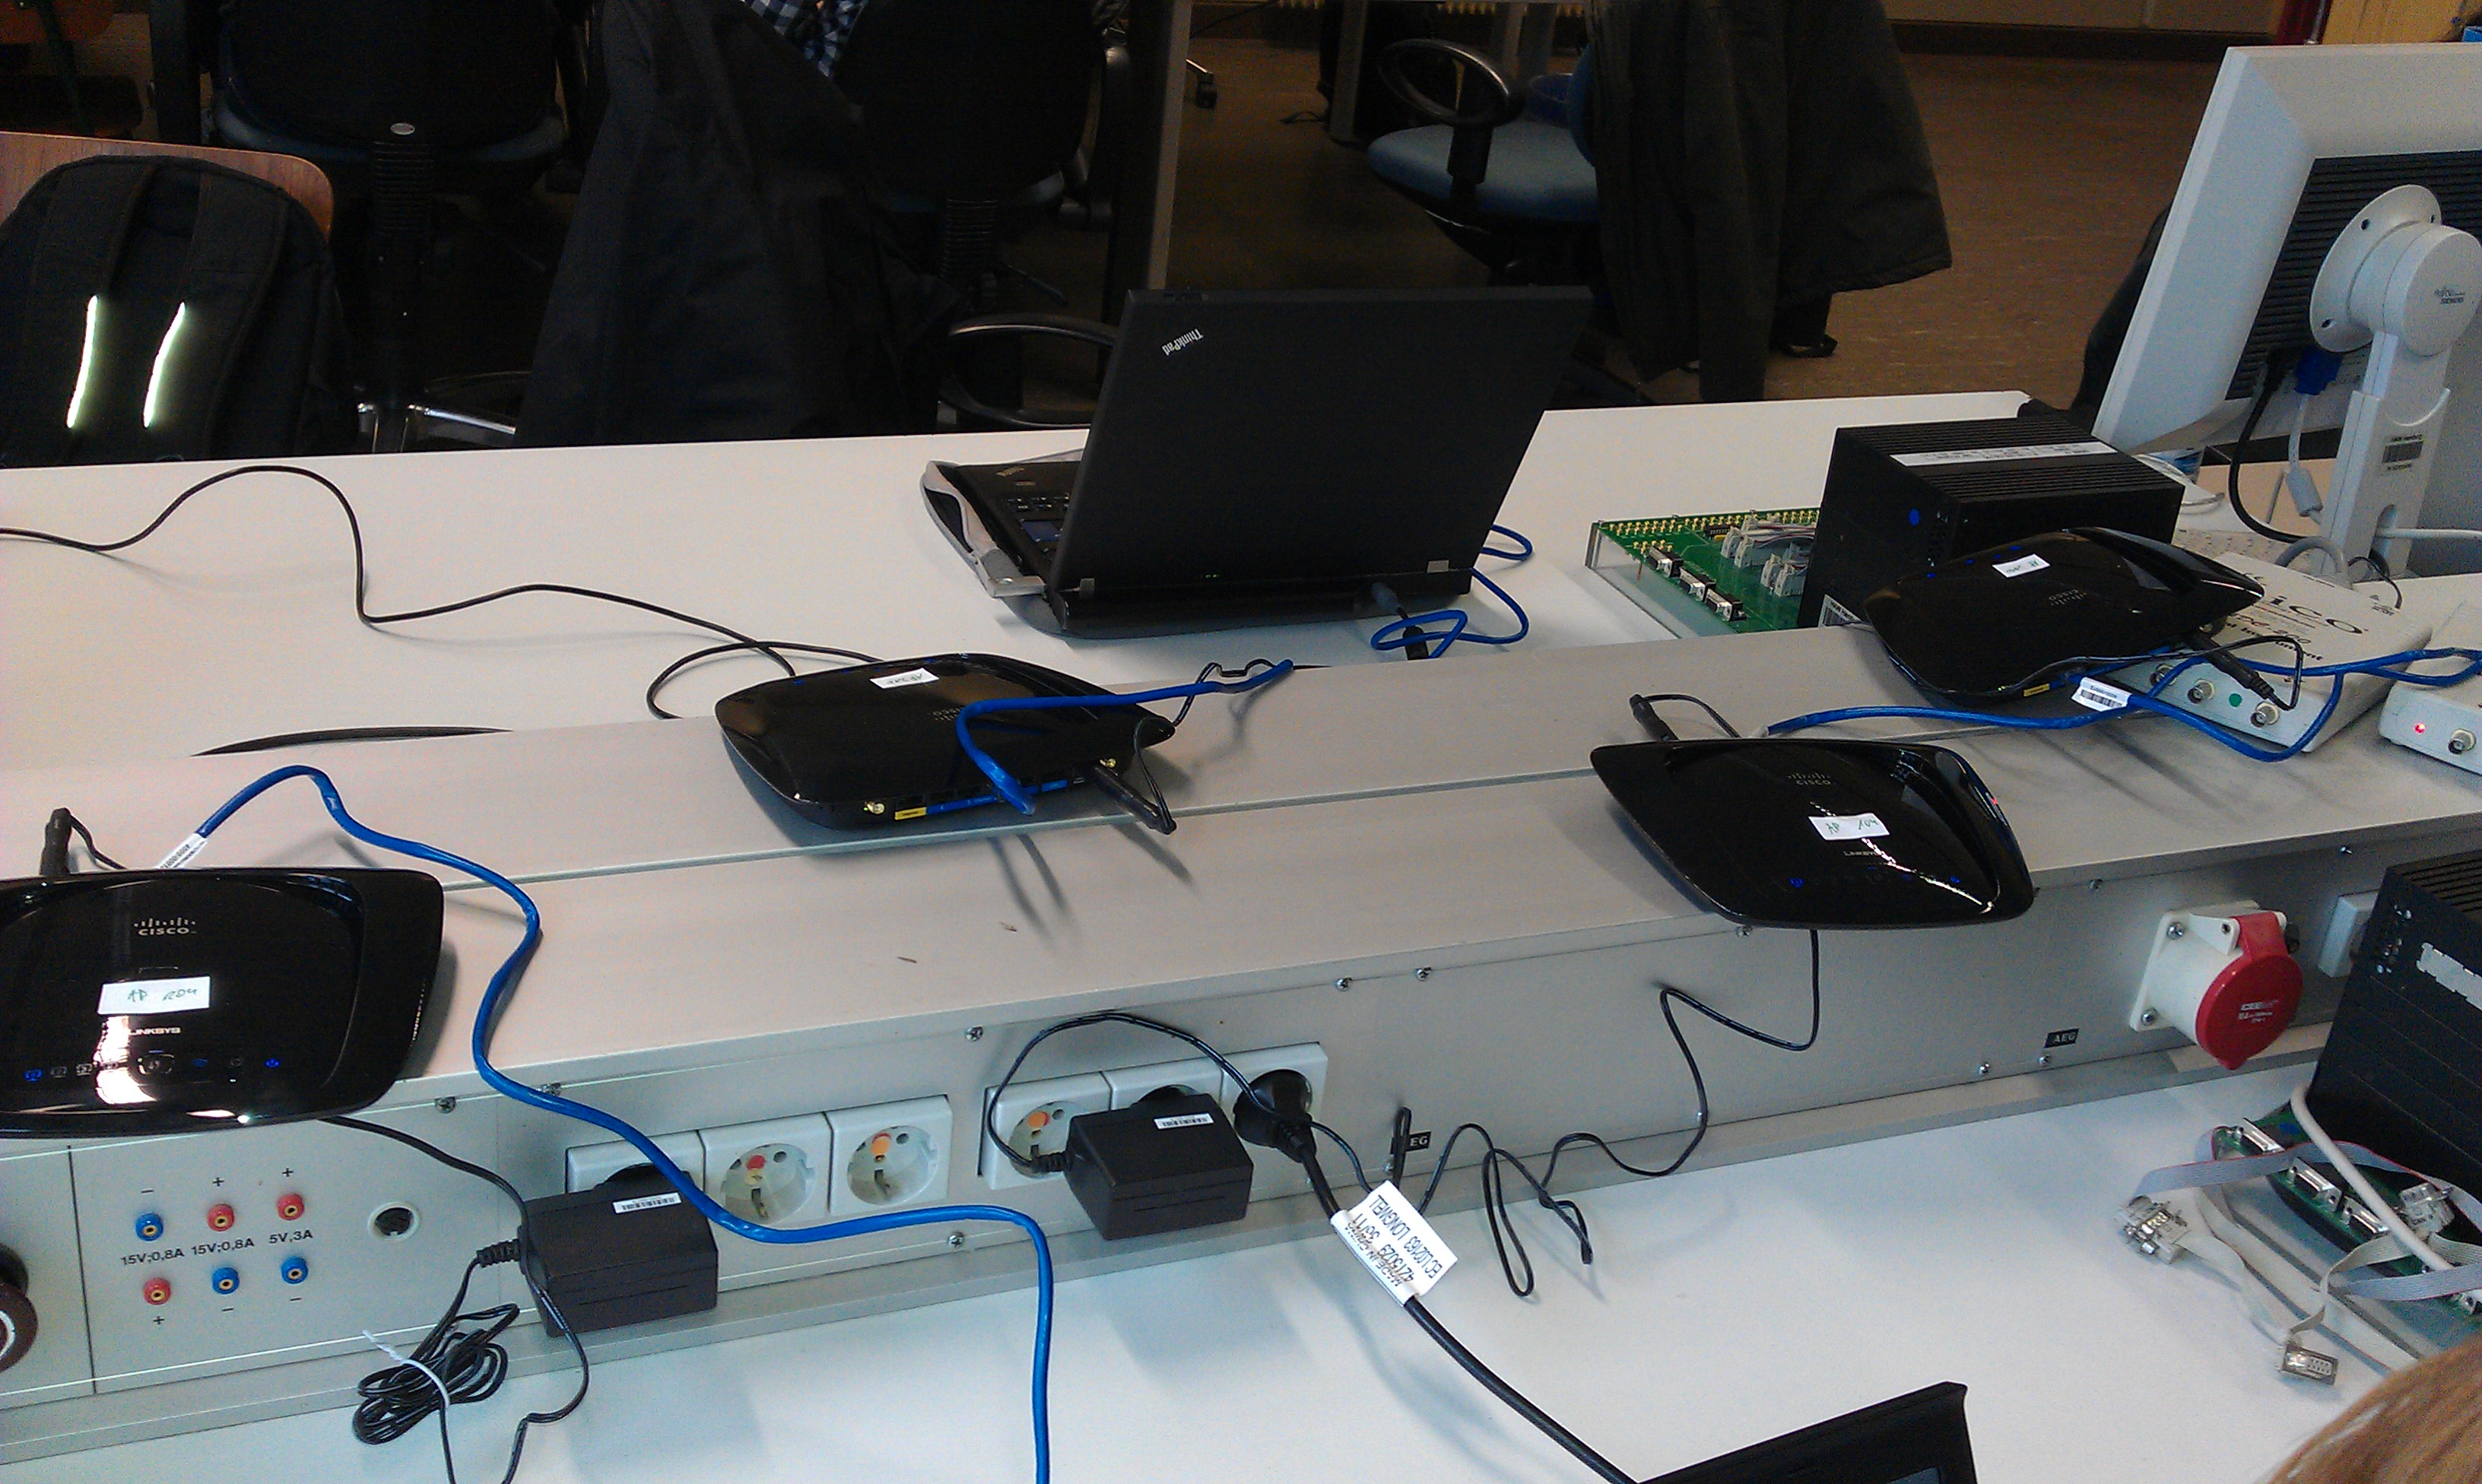
\includegraphics[width=1.0\textwidth]{../AufbauBild.jpg}
	\caption{Versuchsaufbau mit 4 Routern}
	\label{fig:Aufbau}
\end{figure} 

\section{Projektschritt 2 - Vergleich Babel und OLSR}

\subsection{Babel}
\subsubsection{Informationsaustausch}
Jeder Router A hält beim Babel-Protokoll die Kosten zu einem Nachbarrouter B in der Form C(A, B) vor. Die Metrik einer Route bestimmt sich über die Summierung aller Kosten zwischen den Knoten die auf der Route liegen. Das Ziel des Algorithmus liegt darin für jede Quelle S einen Baum der Routen, mit den niedrigsten Metriken zu S zu berechnen.

Babel nutzt \textit{Hello-Messages} zur Durchführung des \textit{Neighbour-Discovery-Processes}.
Hello-Messages werden periodisch über alle Interfaces des Knoten gesendet um so die Nachbarknoten zu entdecken.\\
Zusätzlich werden Hello-Messages in Verbindung mit den \textit{IHY-Messages} (I Heard You Messages) genutzt, um die \textit{Bidirectional Reachability} und die Metrik zwischen Sender- und Empfängerknoten zu ermitteln.
Der Empfänger antwortet auf Hello-Messages mit den IHY-Messages. 
Diese erhalten die, mit Hilfe der Hello-Messages ermittelten, Laufzeitzeitverzögerungen aus Sicht des Senders der Hello-Messages.
Mit Hilfe der Laufzeitverzögerungen findet dann die Bewertung der Qualität der Links, sowohl in Sende- als auch Empfangsrichtung statt.



\subsubsection{Mesh - Konfiguration}
Die lokalen Mesh-Konfigurationen werden über einen verteilten Bellman-Ford Algorithmus berechnetet.\\
Hierzu hält jeder Router A zwei Werte vor, zum einen die geschätzte Distanz zu S (bezeichnet als D(A)) und den Next-Hop-Router zu S (bezeichnet als NH(A)). Zu Beginn des Informationsaustausches ist D(A)=unendlich und NH(A) ist nicht definiert.\\
Periodisch sendet jeder Knoten B ein Update seiner Routen an alle seine Nachbarn mit dem Inhalt D(B), welcher die Distanz zu S angibt. Erhält ein Nachbar A von B ein Update, so prüft A ob B für S als Next-Hop-Router eingetragen ist. Ist dies der Fall wird als Distanz D(A) die Summe aus C(A,B)( = Kosten von A nach B) und D(B)(= Kosten von B zu S) gesetzt. Damit ist im Knoten A die Metrik von A nach S über B aktualisiert.\\
Im Fall, dass B nicht als Next-Hop-Router für S auf A eingetragen ist, vergleicht A die Summe aus C(A,B)( = Kosten von A nach B) und D(B)(= Kosten von B zu S) mit dem gegenwärtigen Wert von D(A). Ist C(A,B)+D(B) kleiner als D(A) ist die angebotene Route besser als die bisher eingetragene und NH(A) wird auf B und D(A) auf C(A,B)+D(B) gesetzt.\\

Im Pseudocode sieht dies in etwa so aus:
\begin{lstlisting}
receiveRouteupdate(D(B)) from B for S
If NH(A) = B Then
	D(A) = C(A,B)+D(B)
Else
	If C(A,B)+D(B) < D(A) Then
		NH(A) = B
		D(A) = C(A,B)+D(B)
	EndIf
EndIf
\end{lstlisting}

Durch den Austausch der Updates wird Mesh-Konfiguration festgelegt und die Knoten wissen an welchen Knoten sie Pakete weiterleiten müssen, um ein bestimmtes Ziel mit möglichst geringen geschätzten Gesamtkosten zu erreichen.

\subsubsection{Loop-Verhinderungsstrategie}
Da es beim Bellman-Ford Algorithmus nach einer Topologieänderung und den damit verbundenen Updates zum \textit{Count-to-infinity}-Problem kommen kann, benötigt Babel eine Loop-Verhinderungs-Strategie.\\
Hierzu werden in Babel die sogenannten \textit{Feasibility Conditions} eingeführt. Dabei werden, erhaltene Routenaktualisierungen verworfen, wenn diese nicht beweisen können, dass die Annahme des Updates zu keinem Loop führen. Router A hält dazu eine \textit{Feasibility Distance} (bezeichnet als FD(A)) vor, welche als Wert die kleinste Distanz zu S enthält, die A jemals angeboten wurde. Ein Update von einem Nachbarn B ist zulässig (feasible), wenn die Metrik D(B) (= Kosten von B zu S) kleiner als As FD(A) ist.\\
Das diese Bedingung weniger restriktiv als die \textit{DSDV-Feasibility} ist, macht das Beispiel in Abbildung \ref{fig:Feasibility} deutlich. A kommt über B zu S, womit D(A)=FD(A)=2 ist. Da D(C)=1 und damit kleiner als FD(A) ist, ist eine alternative Route über C für A zulässig, auch wenn die Metrik C(A,C)+D(C) mit 5 schlechter als die aktuelle Route ist. Für den Fall das die Route über B abbricht kann so die Alternativroute genutzt werden.\\
Die \textit{DSDV-Feasibility} besagt, dass ein Update nur dann angenommen werden darf, wenn C(A,C)+D(C) kleiner oder gleich D(A) ist, wodurch die Alternativroute über C nicht zulässig wäre, da die DSDV-Bedingung nicht erfüllt ist (4+2 $<=$ 2).\\
Um zu zeigen, dass die \textit{Feasibility Condition} trotzdem noch Loop-Freiheit garantiert, sei zu beachten, dass wenn A ein Update von B akzeptiert D(B) nicht kleiner als FD(B) sein kann. Zudem gilt FD(B) ist kleiner als FD(A) da das Update für A zulässig ist und dieser es annimmt. Da diese Eigenschaft weiterhin erhalten bleibt, wenn A Updates versendet, ist sichergestellt, dass die Route keine Loops enthält.

\begin{figure}[htbp]
	\centering	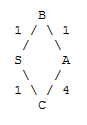
\includegraphics{Grafiken/Feasibility.png}
	\caption{Beispiel Feasabiliy Condition aus \href{http://tools.ietf.org/html/rfc6126}{RFC6126}}
	\label{fig:Feasibility}
\end{figure} 

Um zu verhindern, dass ein Router aufgrund fehlender zulässiger Routen ausgeschlossen wird, werden in Babel die Routen durchnummeriert. Ein Update von B an A ist damit zulässig, wenn entweder die \textit{Feasibility Condition} D(B)$<$FD(A) erfüllt ist und die das Update die gleiche Sequenznummer besitzt oder aber wenn die Sequenznummer des Updates höher ist.


\subsection{OLSR}
\subsubsection{Informationsaustausch}
\subsubsection{Mesh - Konfiguration}
\subsubsection{Loop-Verhinderungsstrategie}

\section{Projektschritt 3 - Vergleich der Übertragungsqualität}

\end{document}

